
\section{Appendix}

Following packages and functions are used in this project.

\begin{Shaded}
\begin{Highlighting}[]
\CommentTok{## basic packages}
\KeywordTok{library}\NormalTok{(knitr)}
\KeywordTok{library}\NormalTok{(kableExtra)}
\KeywordTok{library}\NormalTok{(tidyverse)}
\KeywordTok{library}\NormalTok{(conflicted)}
\KeywordTok{library}\NormalTok{(magrittr)}
\KeywordTok{library}\NormalTok{(broom)}
\CommentTok{# library(car)}
\CommentTok{## paticular packages for this project}
\KeywordTok{library}\NormalTok{(lmtest)}
\KeywordTok{library}\NormalTok{(corrr)}
\KeywordTok{library}\NormalTok{(tseries)}
\KeywordTok{library}\NormalTok{(corrplot)}
\KeywordTok{source}\NormalTok{(}\StringTok{"./funcs.R"}\NormalTok{)}
\end{Highlighting}
\end{Shaded}

The data set is defined as follows based on file \texttt{recs.csv}:

\begin{Shaded}
\begin{Highlighting}[]
\KeywordTok{set.seed}\NormalTok{(}\DecValTok{6}\NormalTok{)}
\NormalTok{dat <-}\StringTok{ }
\StringTok{  }\KeywordTok{read_csv}\NormalTok{(}\StringTok{"./data/recs.csv"}\NormalTok{) }\OperatorTok
\StringTok{  }\NormalTok{dplyr}\OperatorTok{::}\KeywordTok{slice}\NormalTok{(}\KeywordTok{sample}\NormalTok{(}\KeywordTok{nrow}\NormalTok{(.), }\DecValTok{300}\NormalTok{)) }\OperatorTok
\StringTok{  }\KeywordTok{mutate}\NormalTok{(}\DataTypeTok{y =} \KeywordTok{log}\NormalTok{(KWH }\OperatorTok{/}\StringTok{ }\NormalTok{NHSLDMEM)) }\OperatorTok
\StringTok{  }\KeywordTok{mutate}\NormalTok{(}\DataTypeTok{x8 =}\NormalTok{ TOTROOMS }\OperatorTok{+}\StringTok{ }\NormalTok{NCOMBATH }\OperatorTok{+}\StringTok{ }\NormalTok{NHAFBATH) }\OperatorTok
\StringTok{  }\NormalTok{dplyr}\OperatorTok{::}\KeywordTok{select}\NormalTok{(y, }\DataTypeTok{x2 =}\NormalTok{ NHSLDMEM, }\DataTypeTok{x3 =}\NormalTok{ EDUCATION, }\DataTypeTok{x4 =}\NormalTok{ MONEYPY, }\DataTypeTok{x5 =}\NormalTok{ HHSEX, }
    \DataTypeTok{x6 =}\NormalTok{ HHAGE, }\DataTypeTok{x7 =}\NormalTok{ ATHOME, x8) }\OperatorTok
\StringTok{  }\KeywordTok{mutate_at}\NormalTok{(}\KeywordTok{seq}\NormalTok{(}\DecValTok{2}\NormalTok{, }\DecValTok{8}\NormalTok{), as.integer) }\OperatorTok\StringTok{  }\CommentTok{# make continuous variables discrete}
\StringTok{  }\KeywordTok{mutate}\NormalTok{(}\DataTypeTok{x5 =} \OperatorTok{-}\StringTok{ }\NormalTok{x5 }\OperatorTok{+}\StringTok{ }\DecValTok{2}\NormalTok{) }
\end{Highlighting}
\end{Shaded}

\hypertarget{introduction}{%
\subsection{Introduction}\label{introduction}}

Different variables are summarized in the following table. \texttt{y},
the logarithm of averaged electricity consumption, is the variable that
we are interested in. Specifically, The electricity consumption refers
to the electricity usage of the house/studio where the respondent lives
in 2015, measured in kilowatthours. The quantity is average by the
number of household members in the house/studio. That way, it roughly
represent the level of electricity consumption of the respondent. Other
variables are discussion in the following table.

\begin{longtable}[]{@{}lll@{}}
\toprule
Sym & Abbr & Definition\tabularnewline
\midrule
\endhead
z & KWH & electricity consumption\tabularnewline
y & LKWH.pers & logarithm of KWH/NHSLDMEM\tabularnewline
x2 & NHSLDMEM & number of household members\tabularnewline
x3 & EDUCATION & highest education completed\tabularnewline
x4 & MONEYPY & annual gross household income last year\tabularnewline
x5 & HHSEX & gender\tabularnewline
x6 & HHAGE & age\tabularnewline
x7 & ATHOME & number of weekdays someone is at home\tabularnewline
x8 & TOTROOMS + & number of rooms (including bathrooms)\tabularnewline
\bottomrule
\end{longtable}

Note that \texttt{x8} is a variable indicating the number of rooms of
the house/studio of the respondent. It equals the summation of
\texttt{TOTROOMS}, \texttt{NCOMBATH} and \texttt{NHAFBATH} in the
original data set. \texttt{x8} is not included in the initial analysis
(sections 1 to 7).

\texttt{x3}, the education level of the respondent, is considered as a
continuous variable in this project for simplicity. The detailed
definition of different levels is shown in the following table.

\begin{longtable}[]{@{}ll@{}}
\toprule
Level & Definition\tabularnewline
\midrule
\endhead
1 & Less than high school diploma or GED\tabularnewline
2 & High school diploma or GED\tabularnewline
3 & Some college or Associate's degree\tabularnewline
4 & Bachelor's degree (for example: BA, BS)\tabularnewline
5 & Master's, Professional, or Doctorate degree\tabularnewline
\bottomrule
\end{longtable}

The first 5 rows of the data set used can be visualized:

\begin{table}[H]
\centering
\begin{tabular}{llllllll}
\toprule
y & x2 & x3 & x4 & x5 & x6 & x7 & x8\\
\midrule
7.5 & 5 & 3 & 8 & 1 & 39 & 5 & 15\\
8.2 & 1 & 2 & 2 & 0 & 85 & 5 & 14\\
8.7 & 3 & 1 & 1 & 0 & 71 & 5 & 8\\
7.8 & 4 & 3 & 5 & 1 & 39 & 5 & 8\\
9.8 & 1 & 3 & 3 & 0 & 57 & 0 & 10\\
\bottomrule
\end{tabular}
\end{table}

In this project, we want to develop a model associating the continuous
variable, average electricity consumption, with other variables. We will
start by visualizing correlations between variables. In particular, the
two variables \texttt{x2} and \texttt{x6}, which highly correlate with
\texttt{y} will be explored. The model regressing \texttt{y} on
\texttt{x2} will be discussed in section 2. Four assumptions will be
made, three of which will be tested in section 3-5 by Jarque-Bera test
(normality), White's test (homoskedasticity) and RESET test (functional
form) respectively. According the test results and discussion in section
6, data point \texttt{36} is excluded. Then, in section 7, more
regressors are introduced and three new models are established. The
detail regarding how regressors interact with each other, namely
causality, is discussed in section 8. Based on the understanding of the
underlying mechanism, a nonlinear term and \texttt{x8} are included as
new regressors. Two new models are estimated, based on the only model
passing all tests in section 7. Finally, the model called
\texttt{mods{[}{[}7{]}{]}} is chosen as the final for presentation and
it is interpreted in section 10.

\hypertarget{data-visualization}{%
\subsection{Data Visualization}\label{data-visualization}}

It can be seen that \texttt{y} is highly correlated to \texttt{x2} and
\texttt{x6} according to the following table.

\begin{table}[H]
\centering
\begin{tabular}{lll}
\toprule
x & y & r\\
\midrule
x2 & y & -0.511\\
x3 & y & 0.034\\
x4 & y & 0.041\\
x5 & y & -0.043\\
x6 & y & 0.353\\
x7 & y & 0.040\\
x8 & y & 0.213\\
\bottomrule
\end{tabular}
\end{table}

It can be seen from the following covariance matrix that \texttt{y} is
highly correlated to \texttt{x2}, \texttt{x6} and \texttt{x8}. Besides,
\texttt{x3}-\texttt{x4}, \texttt{x2}-\texttt{x6},
\texttt{x4}-\texttt{x8} are high correlated, which will be discussed in
section 9.

\begin{center}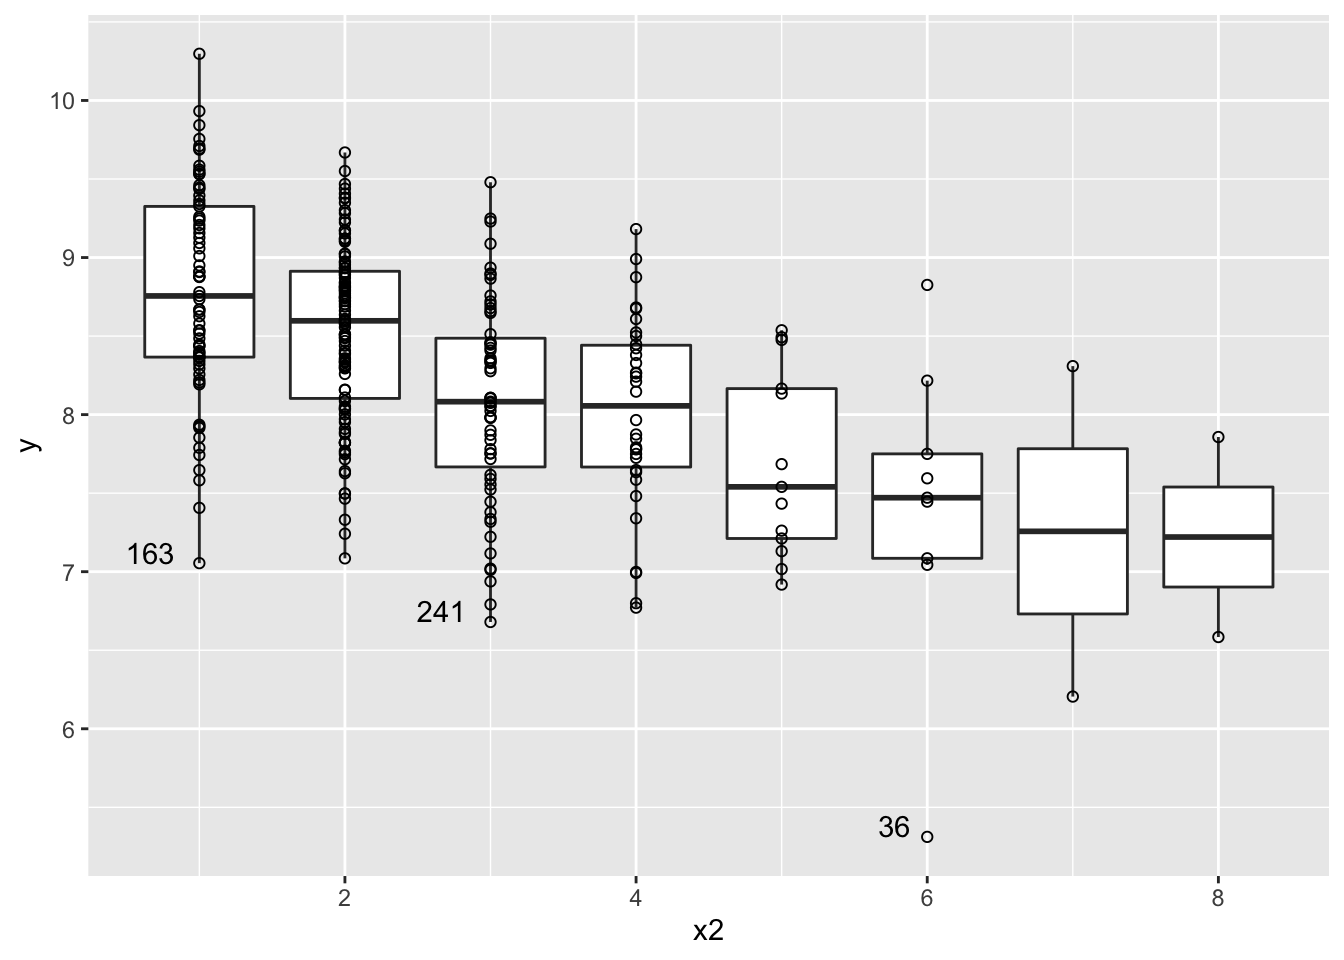
\includegraphics[width=0.48\textwidth]{main_files/figure-latex/unnamed-chunk-7-1} \end{center}

For each level of \texttt{x2} a box indicating three quantiles (25\%,
50\%, 75\%) of \texttt{y} is given. It shows that there is a tendency
for \texttt{y} to decrease with \texttt{x2} by looking at the median.
The sizes of different boxes seem to vary with different values of
\texttt{x2}. Besides, there are many observations when \texttt{x2} is
small. But it is assumed for now that the conditional variance is
constant, which will be tested section 4. Three data points with extreme
values \texttt{36}, \texttt{241} and \texttt{163} is discussed in
sections 3 and 5.

\begin{center}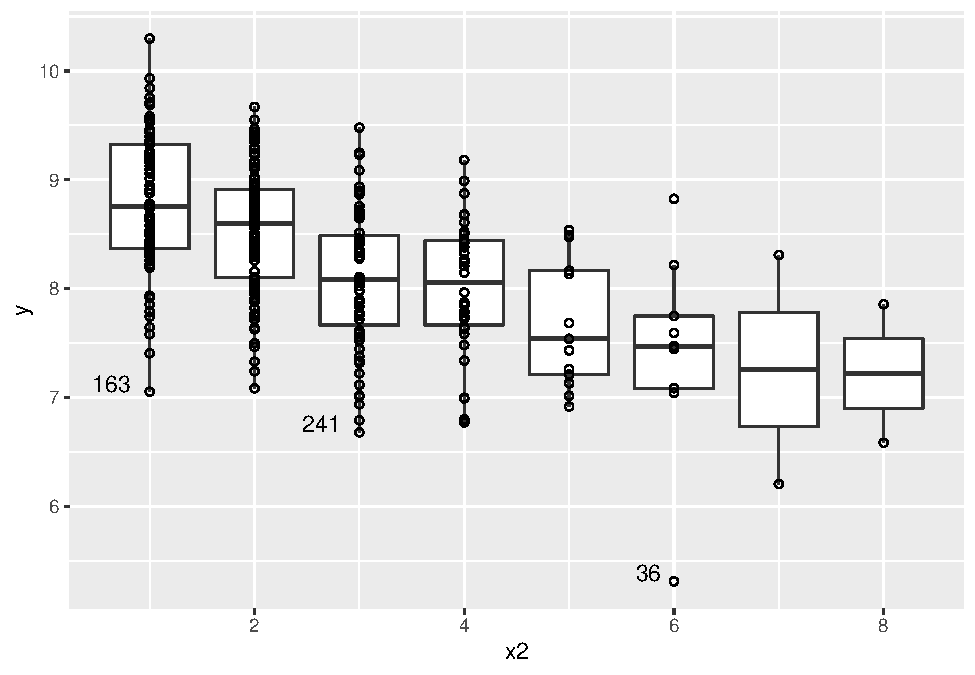
\includegraphics[width=0.48\textwidth]{main_files/figure-latex/unnamed-chunk-8-1} \end{center}

The box plot of \texttt{y} by \texttt{x6} is given. It can be seen that
the tendency is not strictly linear and the condition variance is not
stable. So we will regress \texttt{y} on \texttt{x2} first and use
\texttt{x6} as the second regressor in section 6.

\begin{center}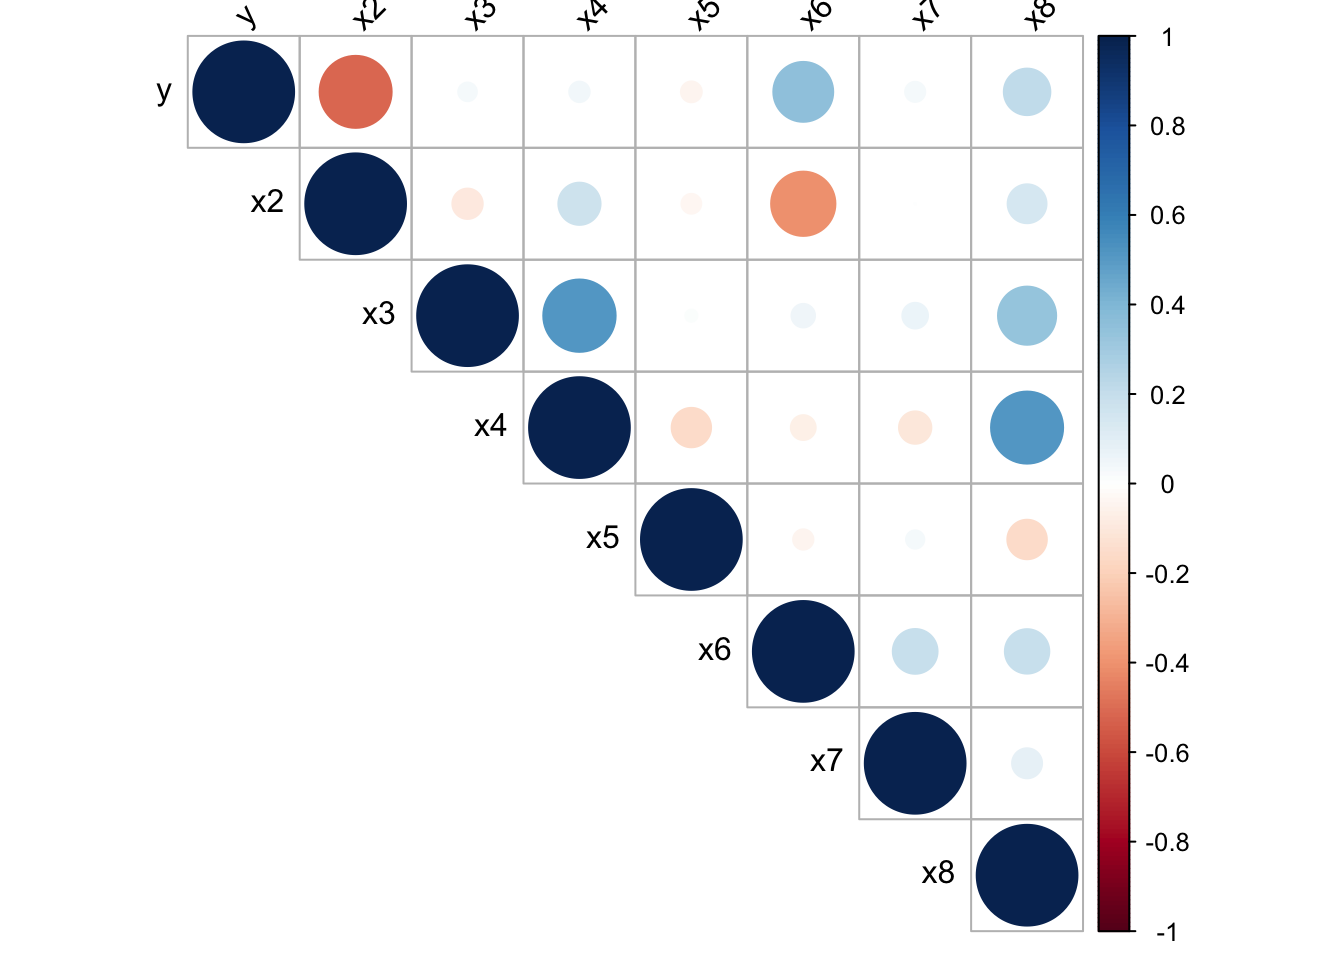
\includegraphics[width=0.48\textwidth]{main_files/figure-latex/unnamed-chunk-9-1} \end{center}

\hypertarget{regress-y-on-x2-assumptions-and-orthogonalization}{%
\subsection{\texorpdfstring{2. Regress \texttt{y} on \texttt{x2},
Assumptions and
Orthogonalization}{2. Regress y on x2, Assumptions and Orthogonalization}}\label{regress-y-on-x2-assumptions-and-orthogonalization}}

\texttt{mods{[}{[}1{]}{]}} is obtained by regressing \texttt{y} on
\texttt{x2}.

\begin{verbatim}
#> lm(formula = y ~ x2, data = dat)
\end{verbatim}

\begin{table}[H]
\centering
\begin{tabular}{lllll}
\toprule
term & estimate & std.error & statistic & p.value\\
\midrule
(Intercept) & 9.04 & 0.075 & 120 & 2.2e-254\\
x2 & -0.27 & 0.026 & -10 & 2.4e-21\\
\bottomrule
\end{tabular}
\end{table}

\begin{table}[H]
\centering
\begin{tabular}{lllllllllll}
\toprule
r.squared & adj.r.squared & sigma & statistic & p.value & df & logLik & AIC & BIC & deviance & df.residual\\
\midrule
0.26 & 0.26 & 0.63 & 105 & 2.4e-21 & 2 & -286 & 579 & 590 & 119 & 298\\
\bottomrule
\end{tabular}
\end{table}

By orthogonalizing \texttt{x2} with respect to constant 1. the following
reparameterized model can be obtained.

\begin{Shaded}
\begin{Highlighting}[]
\NormalTok{mods[[}\DecValTok{2}\NormalTok{]] <-}\StringTok{ }
\StringTok{  }\NormalTok{dat }\OperatorTok
\StringTok{  }\KeywordTok{mutate}\NormalTok{(}\DataTypeTok{x1 =} \DecValTok{1}\NormalTok{, }\DataTypeTok{x21 =}\NormalTok{ x2 }\OperatorTok{-}\StringTok{ }\KeywordTok{mean}\NormalTok{(.}\OperatorTok{$}\NormalTok{x2)) }\OperatorTok
\StringTok{  }\NormalTok{dplyr}\OperatorTok{::}\KeywordTok{select}\NormalTok{(y, x1, x21) }\OperatorTok
\StringTok{  }\NormalTok{\{}\KeywordTok{lm}\NormalTok{(y }\OperatorTok{~}\StringTok{ }\NormalTok{x1 }\OperatorTok{+}\StringTok{ }\NormalTok{x21, }\DataTypeTok{data =}\NormalTok{ .)\}}
\end{Highlighting}
\end{Shaded}

\begin{verbatim}
#> lm(formula = y ~ x1 + x21, data = .)
\end{verbatim}

\begin{table}[H]
\centering
\begin{tabular}{lllll}
\toprule
term & estimate & std.error & statistic & p.value\\
\midrule
(Intercept) & 8.36 & 0.036 & 230 & 0.0e+00\\
x21 & -0.27 & 0.026 & -10 & 2.4e-21\\
\bottomrule
\end{tabular}
\end{table}

\begin{table}[H]
\centering
\begin{tabular}{lllllllllll}
\toprule
r.squared & adj.r.squared & sigma & statistic & p.value & df & logLik & AIC & BIC & deviance & df.residual\\
\midrule
0.26 & 0.26 & 0.63 & 105 & 2.4e-21 & 2 & -286 & 579 & 590 & 119 & 298\\
\bottomrule
\end{tabular}
\end{table}

The estimated regression coefficient for \texttt{x2} in
\texttt{mods{[}{[}1{]}{]}} equals that for \texttt{x21} in
\texttt{mods{[}{[}2{]}{]}}. That is, slopes in these two models are the
same. The standard error of the intercept is reduced by 51.60 \%.
